\documentclass[letterpaper,11pt]{article}

\usepackage{graphicx}
\usepackage{multicol}
\usepackage{fullpage}
\usepackage{csquotes}
\usepackage[margin=0.75in,letterpaper]{geometry}
\setlength{\footskip}{15pt}
\setlength{\belowcaptionskip}{9pt}
\usepackage{censor}
\usepackage{floatflt}
\usepackage{xspace}
\usepackage[margin=1cm,skip=9pt]{caption}
\usepackage{ulem}
\usepackage{tikz}
\usetikzlibrary{shadows}

% https://tex.stackexchange.com/questions/5226/keyboard-font-for-latex
\newcommand*\keys[1]{%
  \tikz[baseline=(key.base)]
    \node[%
      draw,
      fill=white,
      drop shadow={shadow xshift=0.25ex,shadow yshift=-0.25ex,fill=black,opacity=0.75},
      rectangle,
      rounded corners=2pt,
      inner sep=1pt,
      line width=0.5pt,
      minimum width=1.1em,
      font=\scriptsize\sffamily
    ](key) {#1\strut}
  ;
}

\linespread{0.95}
\def\degC{$^{\circ}$C }
\def\degf{$^{\circ}$F }
\def\vol #1 {{\bf #1}, $\;\;$}
\def\refer{\par\noindent\hangindent\parindent\hangafter1}


\title{\vspace{-2.0cm}Herzmann Family Christmas Letter 2023}
\author{Daryl Herzmann${}^1$, Elizabeth Herzmann${}^2$, Margaret 
Herzmann${}^3$,\\
Robert Herzmann${}^3$, AND Charlotte Herzmann${}^3$ \\
\textit{${}^1$Corresponding Author},
\it{${}^2$Responsible Adult},
\it{${}^3$Conscripted Children}}
\date{11 December 2023}

\makeatletter
\newenvironment{tablehere}
  {\def\@captype{table}}
  {}

\newenvironment{figurehere}
  {\def\@captype{figure}}
  {}
\makeatother

\newcommand{\Line}[0]{%
  \rule{0cm}{0cm}\\\hrule\rule{0cm}{0cm}%
}

%\addtolength{\textheight}{1.5in}

\begin{document}
\maketitle
\vspace{-0.75cm}
\begin{abstract}
Behold, the one Christmas Letter that you will actually read and the only one
requiring multiple dictionary consultations to decipher its sesquipedalian prose. 
\end{abstract}

\vspace{-0.5cm}

\noindent\makebox[\linewidth]{\rule{\textwidth}{1pt}}

\begin{multicols}{2}

\section{Materials and Methods} 

Our family comprises Daryl
\enquote{Daryl} (45), Elizabeth \enquote{Liz} (sum of subsequent five prime numbers
greater than 2),
Margaret \enquote{Maggie Moo} (10), Robert \enquote{Bruh} (9), and
Charlotte \enquote{Burger} (6). The cat-shaped void in our hearts persists.

\subsection{Housing and Domestics}

We remain at our permanent house, which will one day serve as our mausoleum.
The only repair was having
both garage door openers conspiculously fail within a week of each other.
We purchased a new couch with a chaise lounge. The chaise is a popular spot for the
children to bond whilst observing screens.

Our lone tree, a once majestic ash, was ravished by the insidious
\emph{Agrilus planipennis}, the emerald ash borer. Figure 1 shows the tree's
demise at the hands of a teenage arboriculturist violating numerous OSHA
regulations.  It has been replaced by a nascent \textit{Liriodendron tulipifera}, tulip tree.
\bigskip

\begin{figurehere}
    \centering   
    \resizebox{.95\columnwidth}{!}{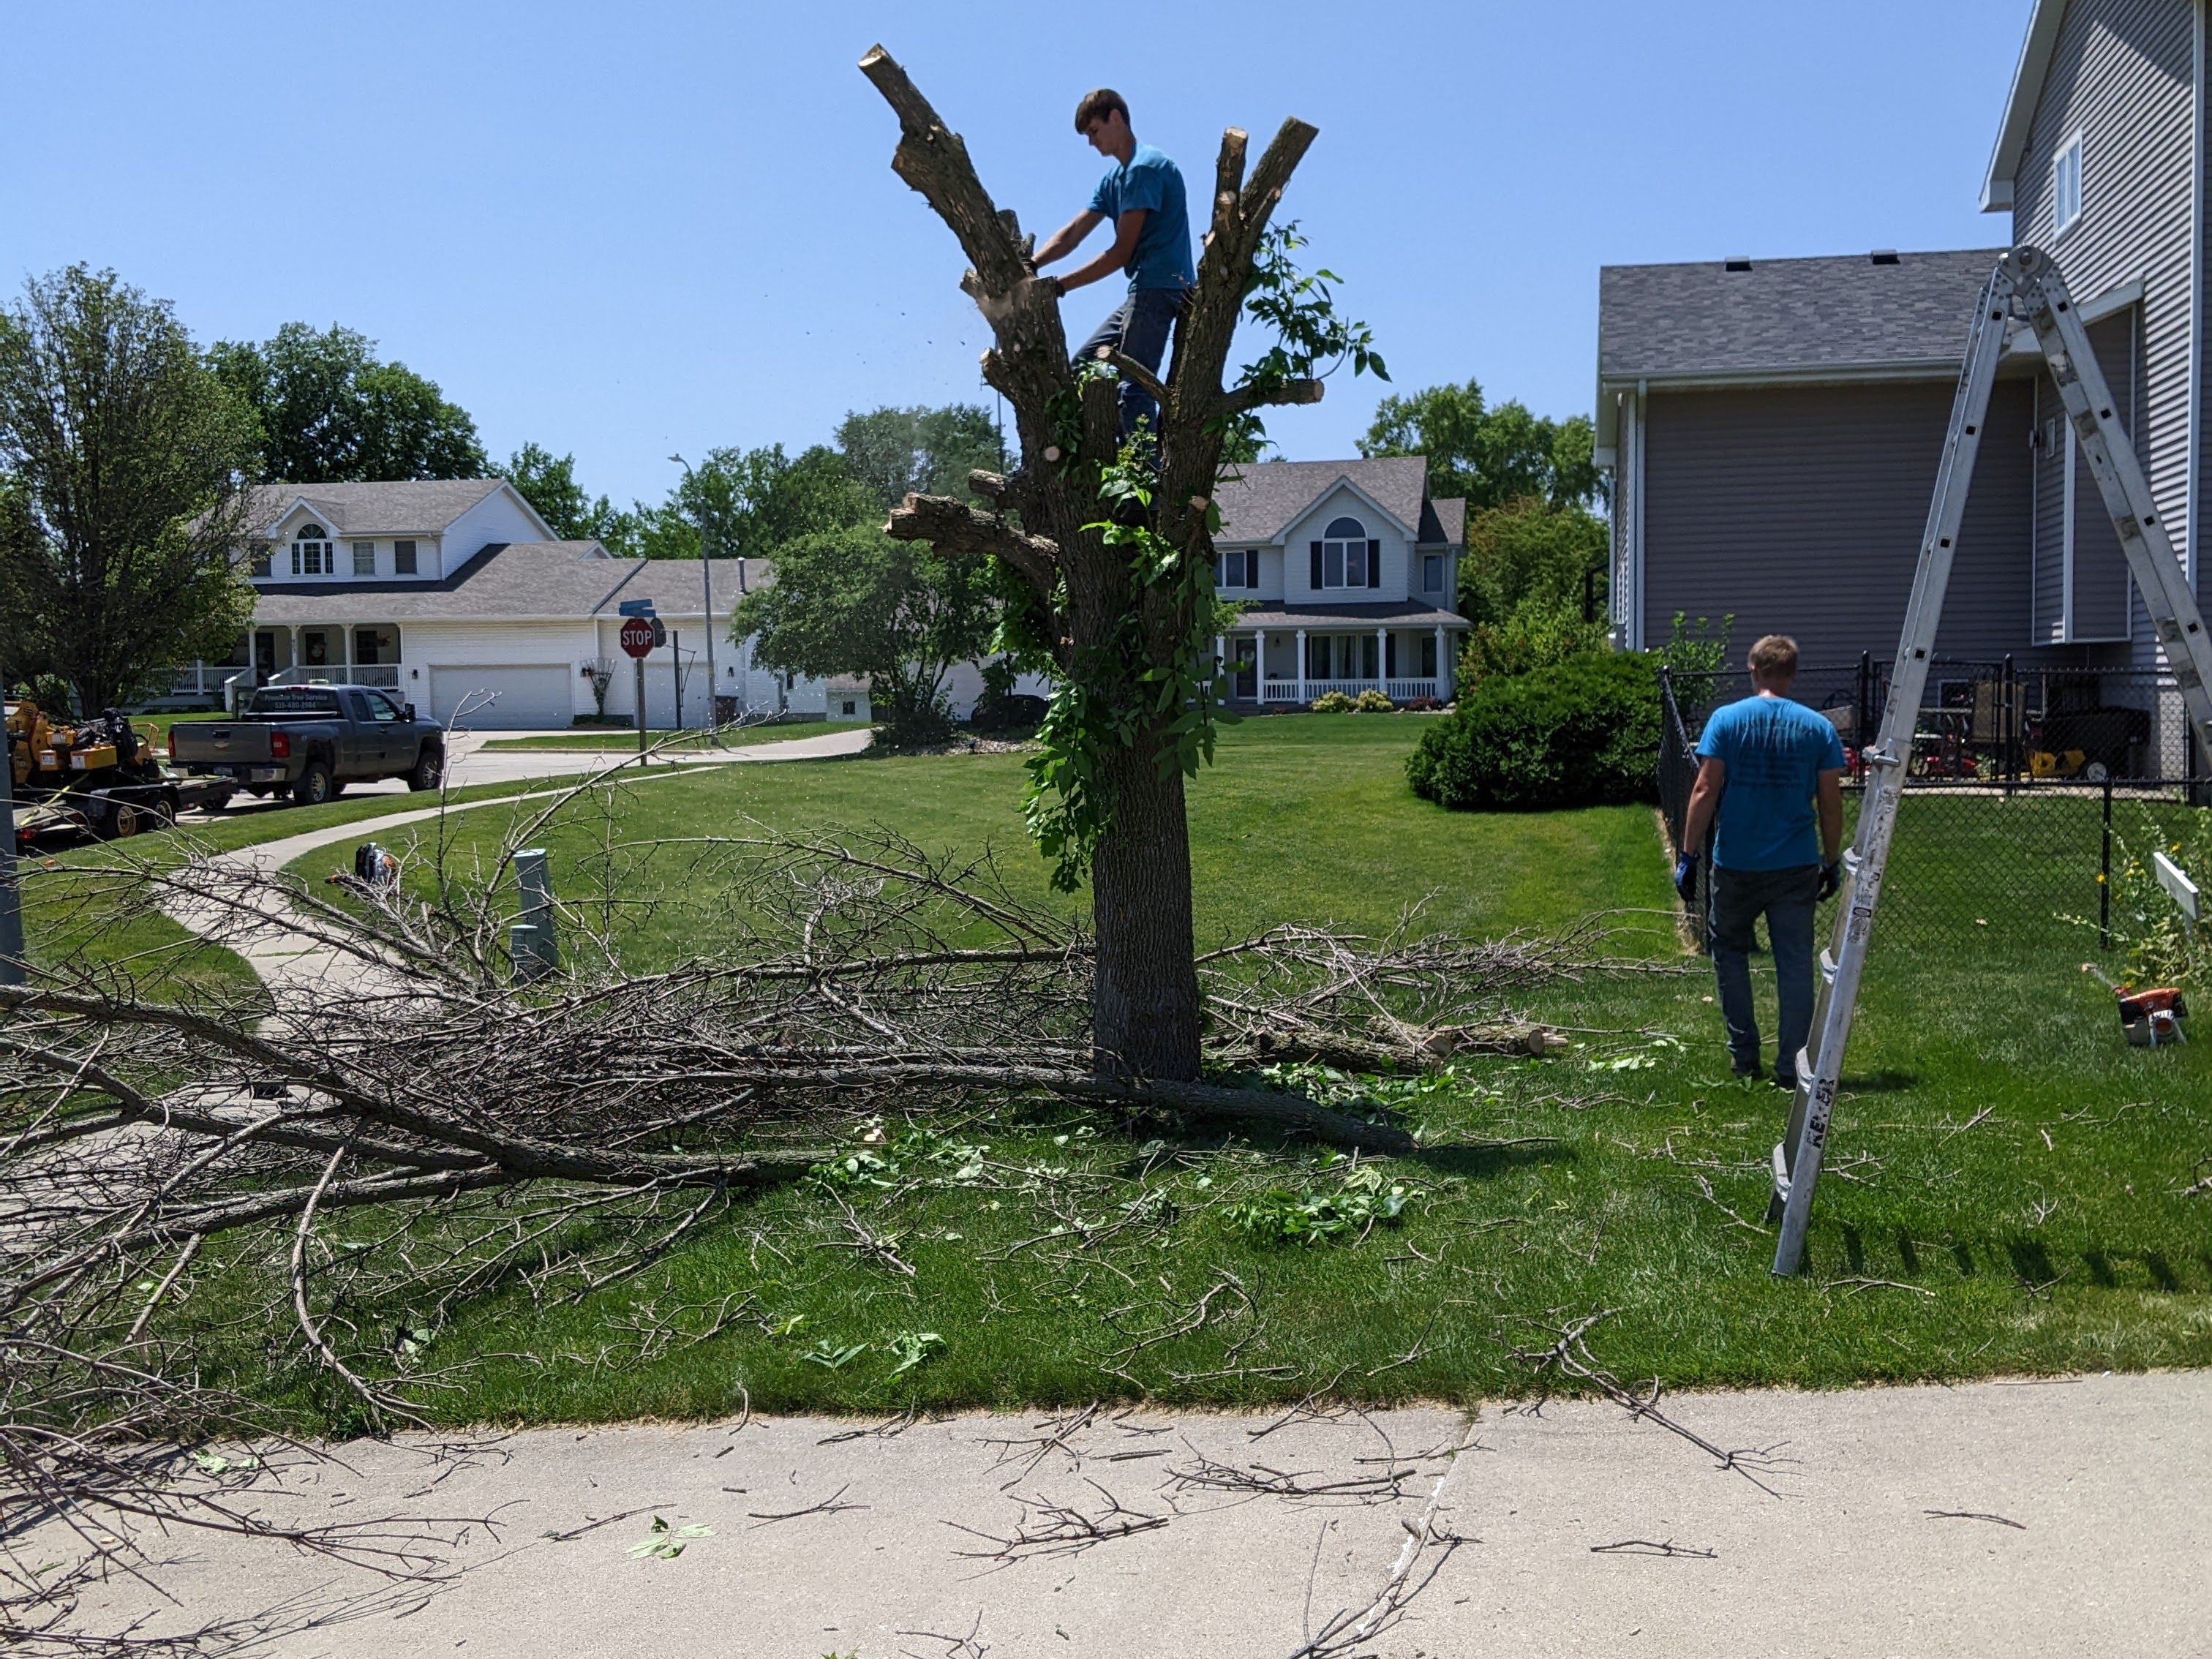
\includegraphics[angle=0]{plots/f1_2023.eps}}
    \caption{Arboricide in action.}
\end{figurehere}


\subsection{Conveyances}

Without neither sufficient funding nor a lottery windfall, we have abandoned prospects of purchasing a
\textit{Ford F150 Lightning}.  For those of you that contributed funds,
they remain in escrow. Our ancient minivan and chaste \textit{Honda Pilot}
will suffice for now. They will also make envious rides for the kids to drive once
they are of legal age and/or the parents get tired of driving them around everywhere.

\bigskip

\subsection{The Matrimonial Partnership}

As of and even after authoring this correspondence, we remain married.  There was a brief scare when a contracted 
Photographic Chronicler posted family photos to \textit{Facebook} without Daryl
included.  Thankfully, Photoshop was able to rectify the situation.

Daryl experienced multiple mid-life crises after deciding to train
for a marathon (Figure 2), which included growing long hair.
Schadenfreudian pleasure is still found with his daily automotive purgatory commute
to the altar of productivity at Iowa State University.

\begin{figurehere}
    \centering   
    \resizebox{.95\columnwidth}{!}{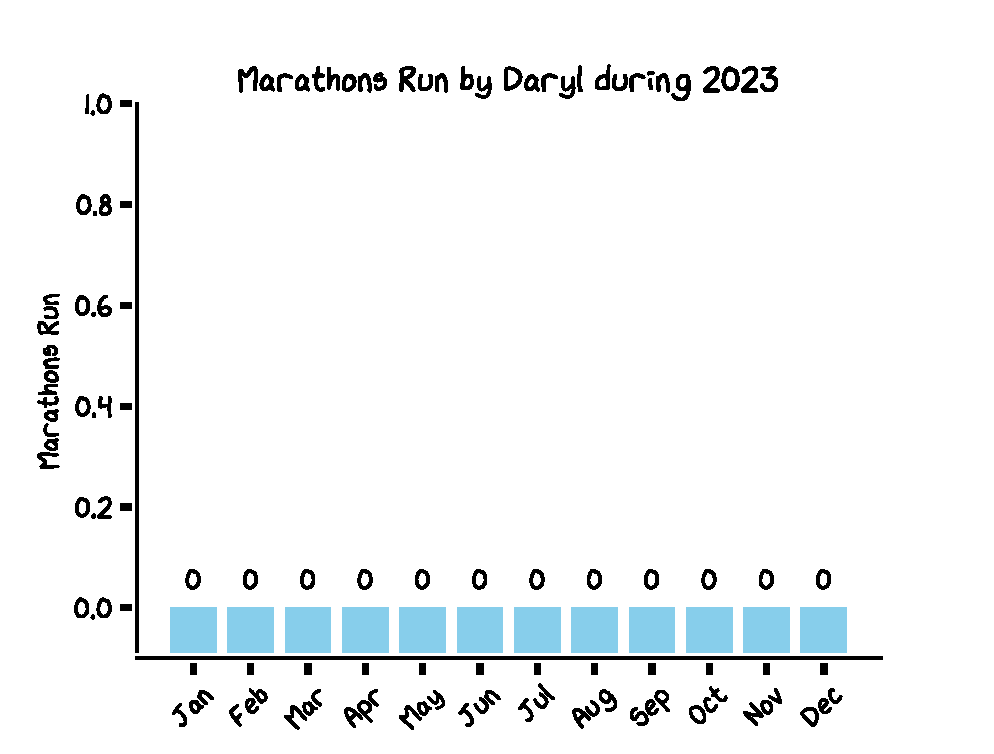
\includegraphics[angle=0]{plots/f2_2023.eps}}
    \caption{Prodiguous training result.}
\end{figurehere}

Liz denotes that nothing of consequence has changed in her life over the past
year. She still teaches at Southview Middle School here in Ankeny and allocates
all other time to the children.

\section{Miss Charlotte}

Charlotte opines: \texttt{I love my mom and dad. I like going on trips, it's the best.
I do a sport. I like to read \textit{Dogman}. I like ${1}^{st}$ grade. I love you.}
To elaborate slightly, she
very much enjoys school and spending time with her friends.  She likes soccer and
will be trying basketball and volleyball soon. As her great-grandmother's namesake,
she continues to be a fiery and loving spirit.

\section{Mr Robert}

${4}^{th}$ grader Robert wanted an AI to creatively phrase his activities:
Robert's leisure activities include digital recreation, with a 
preference for the competitive platform known as \textit{Brawl Stars}. This
virtual environment provides an outlet for his strategic thinking and
competitive spirit. He demonstrates sustained engagement in the sonic arts,
specifically focusing on the piano. This dedication was recently showcased
during a public performance. He has also shown a strong affinity for the written
word, particularly the magical world of \textit{Harry Potter} and the humorous insights
of \textit{Calvin and Hobbes}.

\section{Miss Maggie}

I’m in ${5}^{th}$ grade, my last year of elementary school. I got the
opportunity to start band at school and I have now played clarinet in one out
of my two band concerts. I got the opportunity to lead my school's
\textquotedblleft{\textit{Awesome Assembly}}\textquotedblright. I am also in yearbook club again. Outside of school,
I continue to play volleyball and now am on an Ankeny volleyball team (AVBA).
I continue to fulfill my passion of dancing and was in my 3rd nutcracker
performance. This year I rocked being a ballerina doll, Russian dancer, and a
flower in \textit{The Nutcracker}. I found a new passion of crocheting and have made a
chicken, penguin, and a whale. I also recently got into graphic design and made
the family Christmas card this year. I will again this year request toiletry
items [editorial: to donate, not that parents fail to provide such things] instead of birthday presents for my ${11}^{th}$ birthday in January. --- Love Maggie

\section{Family Trips}

We took a spring break expedition to the vibrant metropolis of St. Louis.
Being at the top of the Gateway Arch on a windy day offered a more nauseating
than usual view of the city.  We explored the
Meramec Caverns, which was a much different experience than previous
claustrophobic ventures underground.

Our family vacation trip was to Yooper Michigan, specifically Munising (Figure 3), in
August.  We were filled with disquietude to learn that the \textit{Edmund Fitzgerald} was not
destined for Cleveland as sung by Lightfoot (1976), but rather was headed to
Detroit.  This was apropos, sans the wreck, for our return trip home as Liz and the kids
disembarked in Cedar Rapids by the airlines as Daryl raced them to Des
Moines in the minivan.  The kids got an authentic first experience of the
horrors of airline travel.

\bigskip

\begin{figurehere}
    \centering   
    \resizebox{.95\columnwidth}{!}{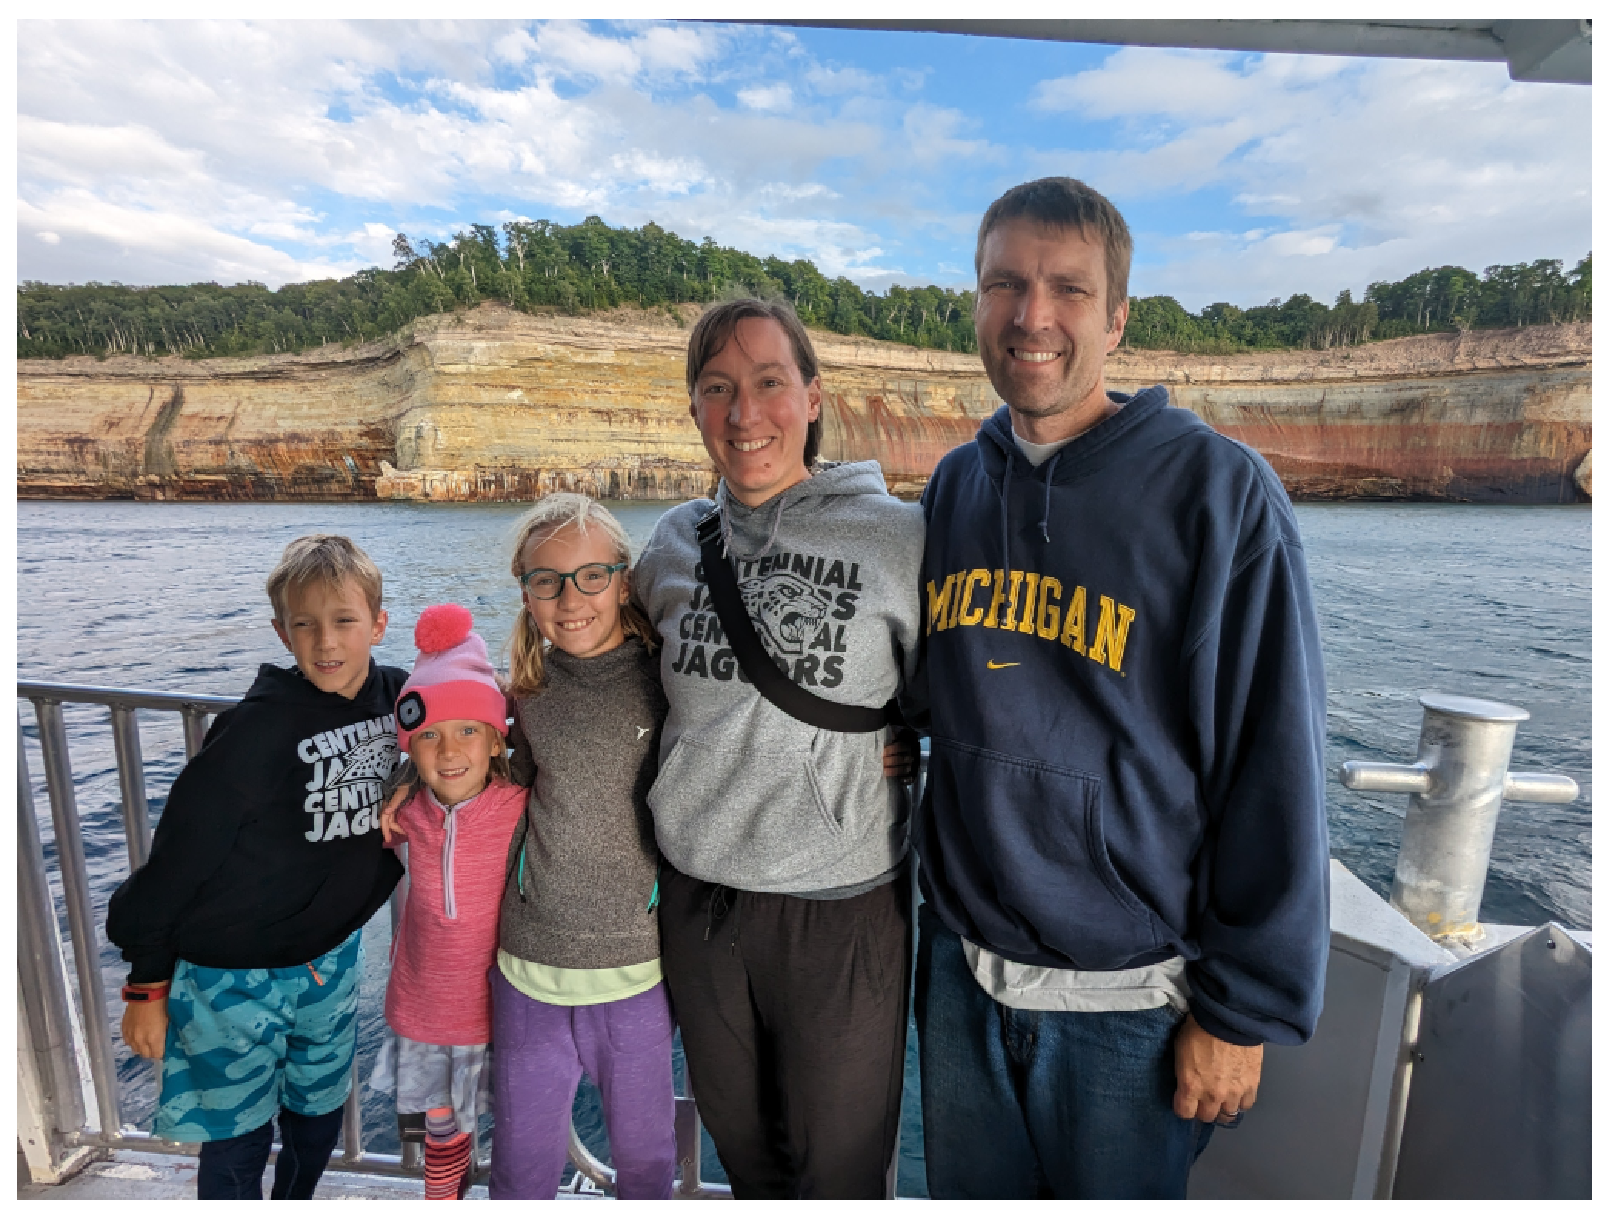
\includegraphics[angle=0]{plots/f3_2023.eps}}
    \caption{Family pictured in front of Pictured Rocks National Lakeshore.}
\end{figurehere}

\bigskip

\emph{Acknowledgments} Our family wishes to thank you for the generous 
support, prayers, cards, gifts, and visits you have provided us in the past
year. Color page charges associated with this missive may preclude the children
from attending college. AI attempted to tone down my rhetoric, but failed. Full
\LaTeX\xspace source of this letter can be found on Daryl's Github page. 

\section{References}

\refer Github, 2023: \texttt{https://github.com/akrherz/akrherz}, last viewed on 9 Dec 2023.
\refer Lightfoot, Gordon. "The Wreck of the Edmund Fitzgerald." \emph{Summertime Dream}, Reprise Records, 1976.

\end{multicols}

\end{document}
